% Options for packages loaded elsewhere
\PassOptionsToPackage{unicode}{hyperref}
\PassOptionsToPackage{hyphens}{url}
%
\documentclass[
  10pt,
  a4paper,
]{article}
\usepackage{amsmath,amssymb}
\usepackage{iftex}
\ifPDFTeX
  \usepackage[T1]{fontenc}
  \usepackage[utf8]{inputenc}
  \usepackage{textcomp} % provide euro and other symbols
\else % if luatex or xetex
  \usepackage{unicode-math} % this also loads fontspec
  \defaultfontfeatures{Scale=MatchLowercase}
  \defaultfontfeatures[\rmfamily]{Ligatures=TeX,Scale=1}
\fi
\usepackage{lmodern}
\ifPDFTeX\else
  % xetex/luatex font selection
  \setmainfont[]{DejaVu Sans}
  \setmonofont[]{DejaVu Sans Mono}
\fi
% Use upquote if available, for straight quotes in verbatim environments
\IfFileExists{upquote.sty}{\usepackage{upquote}}{}
\IfFileExists{microtype.sty}{% use microtype if available
  \usepackage[]{microtype}
  \UseMicrotypeSet[protrusion]{basicmath} % disable protrusion for tt fonts
}{}
\makeatletter
\@ifundefined{KOMAClassName}{% if non-KOMA class
  \IfFileExists{parskip.sty}{%
    \usepackage{parskip}
  }{% else
    \setlength{\parindent}{0pt}
    \setlength{\parskip}{6pt plus 2pt minus 1pt}}
}{% if KOMA class
  \KOMAoptions{parskip=half}}
\makeatother
\usepackage{xcolor}
\usepackage[margin=19mm]{geometry}
\usepackage{color}
\usepackage{fancyvrb}
\newcommand{\VerbBar}{|}
\newcommand{\VERB}{\Verb[commandchars=\\\{\}]}
\DefineVerbatimEnvironment{Highlighting}{Verbatim}{commandchars=\\\{\}}
% Add ',fontsize=\small' for more characters per line
\newenvironment{Shaded}{}{}
\newcommand{\AlertTok}[1]{\textcolor[rgb]{1.00,0.00,0.00}{\textbf{#1}}}
\newcommand{\AnnotationTok}[1]{\textcolor[rgb]{0.38,0.63,0.69}{\textbf{\textit{#1}}}}
\newcommand{\AttributeTok}[1]{\textcolor[rgb]{0.49,0.56,0.16}{#1}}
\newcommand{\BaseNTok}[1]{\textcolor[rgb]{0.25,0.63,0.44}{#1}}
\newcommand{\BuiltInTok}[1]{\textcolor[rgb]{0.00,0.50,0.00}{#1}}
\newcommand{\CharTok}[1]{\textcolor[rgb]{0.25,0.44,0.63}{#1}}
\newcommand{\CommentTok}[1]{\textcolor[rgb]{0.38,0.63,0.69}{\textit{#1}}}
\newcommand{\CommentVarTok}[1]{\textcolor[rgb]{0.38,0.63,0.69}{\textbf{\textit{#1}}}}
\newcommand{\ConstantTok}[1]{\textcolor[rgb]{0.53,0.00,0.00}{#1}}
\newcommand{\ControlFlowTok}[1]{\textcolor[rgb]{0.00,0.44,0.13}{\textbf{#1}}}
\newcommand{\DataTypeTok}[1]{\textcolor[rgb]{0.56,0.13,0.00}{#1}}
\newcommand{\DecValTok}[1]{\textcolor[rgb]{0.25,0.63,0.44}{#1}}
\newcommand{\DocumentationTok}[1]{\textcolor[rgb]{0.73,0.13,0.13}{\textit{#1}}}
\newcommand{\ErrorTok}[1]{\textcolor[rgb]{1.00,0.00,0.00}{\textbf{#1}}}
\newcommand{\ExtensionTok}[1]{#1}
\newcommand{\FloatTok}[1]{\textcolor[rgb]{0.25,0.63,0.44}{#1}}
\newcommand{\FunctionTok}[1]{\textcolor[rgb]{0.02,0.16,0.49}{#1}}
\newcommand{\ImportTok}[1]{\textcolor[rgb]{0.00,0.50,0.00}{\textbf{#1}}}
\newcommand{\InformationTok}[1]{\textcolor[rgb]{0.38,0.63,0.69}{\textbf{\textit{#1}}}}
\newcommand{\KeywordTok}[1]{\textcolor[rgb]{0.00,0.44,0.13}{\textbf{#1}}}
\newcommand{\NormalTok}[1]{#1}
\newcommand{\OperatorTok}[1]{\textcolor[rgb]{0.40,0.40,0.40}{#1}}
\newcommand{\OtherTok}[1]{\textcolor[rgb]{0.00,0.44,0.13}{#1}}
\newcommand{\PreprocessorTok}[1]{\textcolor[rgb]{0.74,0.48,0.00}{#1}}
\newcommand{\RegionMarkerTok}[1]{#1}
\newcommand{\SpecialCharTok}[1]{\textcolor[rgb]{0.25,0.44,0.63}{#1}}
\newcommand{\SpecialStringTok}[1]{\textcolor[rgb]{0.73,0.40,0.53}{#1}}
\newcommand{\StringTok}[1]{\textcolor[rgb]{0.25,0.44,0.63}{#1}}
\newcommand{\VariableTok}[1]{\textcolor[rgb]{0.10,0.09,0.49}{#1}}
\newcommand{\VerbatimStringTok}[1]{\textcolor[rgb]{0.25,0.44,0.63}{#1}}
\newcommand{\WarningTok}[1]{\textcolor[rgb]{0.38,0.63,0.69}{\textbf{\textit{#1}}}}
\usepackage{longtable,booktabs,array}
\usepackage{calc} % for calculating minipage widths
% Correct order of tables after \paragraph or \subparagraph
\usepackage{etoolbox}
\makeatletter
\patchcmd\longtable{\par}{\if@noskipsec\mbox{}\fi\par}{}{}
\makeatother
% Allow footnotes in longtable head/foot
\IfFileExists{footnotehyper.sty}{\usepackage{footnotehyper}}{\usepackage{footnote}}
\makesavenoteenv{longtable}
\usepackage{graphicx}
\makeatletter
\def\maxwidth{\ifdim\Gin@nat@width>\linewidth\linewidth\else\Gin@nat@width\fi}
\def\maxheight{\ifdim\Gin@nat@height>\textheight\textheight\else\Gin@nat@height\fi}
\makeatother
% Scale images if necessary, so that they will not overflow the page
% margins by default, and it is still possible to overwrite the defaults
% using explicit options in \includegraphics[width, height, ...]{}
\setkeys{Gin}{width=\maxwidth,height=\maxheight,keepaspectratio}
% Set default figure placement to htbp
\makeatletter
\def\fps@figure{htbp}
\makeatother
\setlength{\emergencystretch}{3em} % prevent overfull lines
\providecommand{\tightlist}{%
  \setlength{\itemsep}{0pt}\setlength{\parskip}{0pt}}
\setcounter{secnumdepth}{-\maxdimen} % remove section numbering
\ifLuaTeX
\usepackage[bidi=basic]{babel}
\else
\usepackage[bidi=default]{babel}
\fi
\babelprovide[main,import]{french}
\ifPDFTeX
\else
\babelfont{rm}[]{DejaVu Sans}
\fi
% get rid of language-specific shorthands (see #6817):
\let\LanguageShortHands\languageshorthands
\def\languageshorthands#1{}
\usepackage{etoolbox}
\usepackage{microtype}
\usepackage{float}
\floatplacement{figure}{H}
\setlength{\emergencystretch}{3em}
\setlength{\parskip}{0.35em}
\AtBeginEnvironment{longtable}{\small}
\AtBeginDocument{\hypersetup{colorlinks=true,linkcolor=blue!45!black,urlcolor=blue!45!black}}
\ifLuaTeX
  \usepackage{selnolig}  % disable illegal ligatures
\fi
\IfFileExists{bookmark.sty}{\usepackage{bookmark}}{\usepackage{hyperref}}
\IfFileExists{xurl.sty}{\usepackage{xurl}}{} % add URL line breaks if available
\urlstyle{same}
\hypersetup{
  pdflang={fr-FR},
  hidelinks,
  pdfcreator={LaTeX via pandoc}}

\author{}
\date{}

\begin{document}

\hypertarget{v6.41-fibres-plis-et-positivituxe9-le-graphe-des-passages}{%
\section{V6.41 --- Fibres, plis et positivité : le graphe des
passages}\label{v6.41-fibres-plis-et-positivituxe9-le-graphe-des-passages}}

\textbf{Document 65 · Vincent P. P. NOËL · 12 octobre 2026}

Note de recherche et dossier LaTeX. Démonstrations auxiliaires,
expériences prospectives et deux relectures internes confrontées.

\hypertarget{la-clef-locale-trouvuxe9e-la-clef-globale-encore-cherchuxe9e}{%
\subsection{1. La clef locale trouvée, la clef globale encore
cherchée}\label{la-clef-locale-trouvuxe9e-la-clef-globale-encore-cherchuxe9e}}

\textbf{La destination logique est connue : RH. Le chemin de preuve
reste à construire.} RH affirme que tous les zéros non triviaux de ζ ont
partie réelle 1/2. Une autre « destination » peut désigner l'objet
intermédiaire qui ferait réussir une preuve : nous en fixons deux, avec
leurs quantificateurs et leur implication finale.

Le changement d'objet utile est de suivre \textbf{la paire de zéros},
son centre et son discriminant, au lieu de conserver à tout prix le nom
de chacun des deux zéros. Au point double, les étiquettes deviennent
ambiguës ; la paire non ordonnée possède encore un polynôme et un
opérateur compagnon. Sous un contour isolant, les moments les
reconstruisent sans choix de branche. Cette clef locale n'est pas une
preuve de positivité globale.

\begin{longtable}[]{@{}
  >{\raggedright\arraybackslash}p{(\columnwidth - 4\tabcolsep) * \real{0.3333}}
  >{\raggedright\arraybackslash}p{(\columnwidth - 4\tabcolsep) * \real{0.3333}}
  >{\raggedright\arraybackslash}p{(\columnwidth - 4\tabcolsep) * \real{0.3333}}@{}}
\toprule\noalign{}
\begin{minipage}[b]{\linewidth}\raggedright
Obstacle précédent
\end{minipage} & \begin{minipage}[b]{\linewidth}\raggedright
Acquis V6.41
\end{minipage} & \begin{minipage}[b]{\linewidth}\raggedright
Ce qui reste ouvert
\end{minipage} \\
\midrule\noalign{}
\endhead
\bottomrule\noalign{}
\endlastfoot
A complexe prescrit & Test exact de faisabilité : ellipse ; fibre S²,
singleton ou vide & Aucune affirmation d'accessibilité de tout le plan
complexe à ancre et rayon fixés \\
D varie-t-il toujours à A fixé ? & Non : A=0 donne D≡1 ; variation
générique démontrée à l'intérieur & Aucun sens uniforme du mouvement des
zéros n'en découle \\
Zéros critiques doubles & Théorème conditionnel du pli ; 20 candidats
recoupés, six attribués aux branches suivies & Existence et unicité
certifiées par intervalles ; autres collisions et hauteurs \\
Passage entre branches & Paire sans étiquette, moments, discriminant et
compagnon ; 18 blocs reconstruits & Contours continus isolants et
couverture exhaustive non certifiés \\
Positivité liée à RH & Tests admissibles, densité, obstruction aux seuls
préfixes finis, budget de Schur & Identité arithmétique et estimations
uniformes pour ζ \\
\end{longtable}

Les calculs sont annoncés comme des recoupements numériques. Le
certificat par intervalles présent concerne les sommes finies de phases
et la géométrie de A=0 ; il ne certifie pas les zéros des fonctions L.

\textbf{Deux portes vers RH.} Porte 1 : prouver la positivité de la
forme arithmétique de Weil sur chaque test admissible. Porte 2 : obtenir
directement depuis les nombres premiers une borne \(Q(X)=X^{o(1)}\),
puis appliquer le théorème A du corpus. Les résultats locaux ci-dessous
ne fournissent encore ni l'une ni l'autre.

Fermer une voie sous des hypothèses précises est un progrès de
discrimination. Cela n'établit pas l'inexistence de tout chemin vers RH.
Les noms « théorème » et « lemme » désignent ici des énoncés accompagnés
de preuves dans le corpus, avec relecture interne ; ils ne désignent pas
une validation externe nouvelle.

\newpage

\hypertarget{le-graphe-ce-qui-muxe8ne-uxe0-quoi}{%
\subsection{2. Le graphe : ce qui mène à
quoi}\label{le-graphe-ce-qui-muxe8ne-uxe0-quoi}}

\begin{figure}
\centering
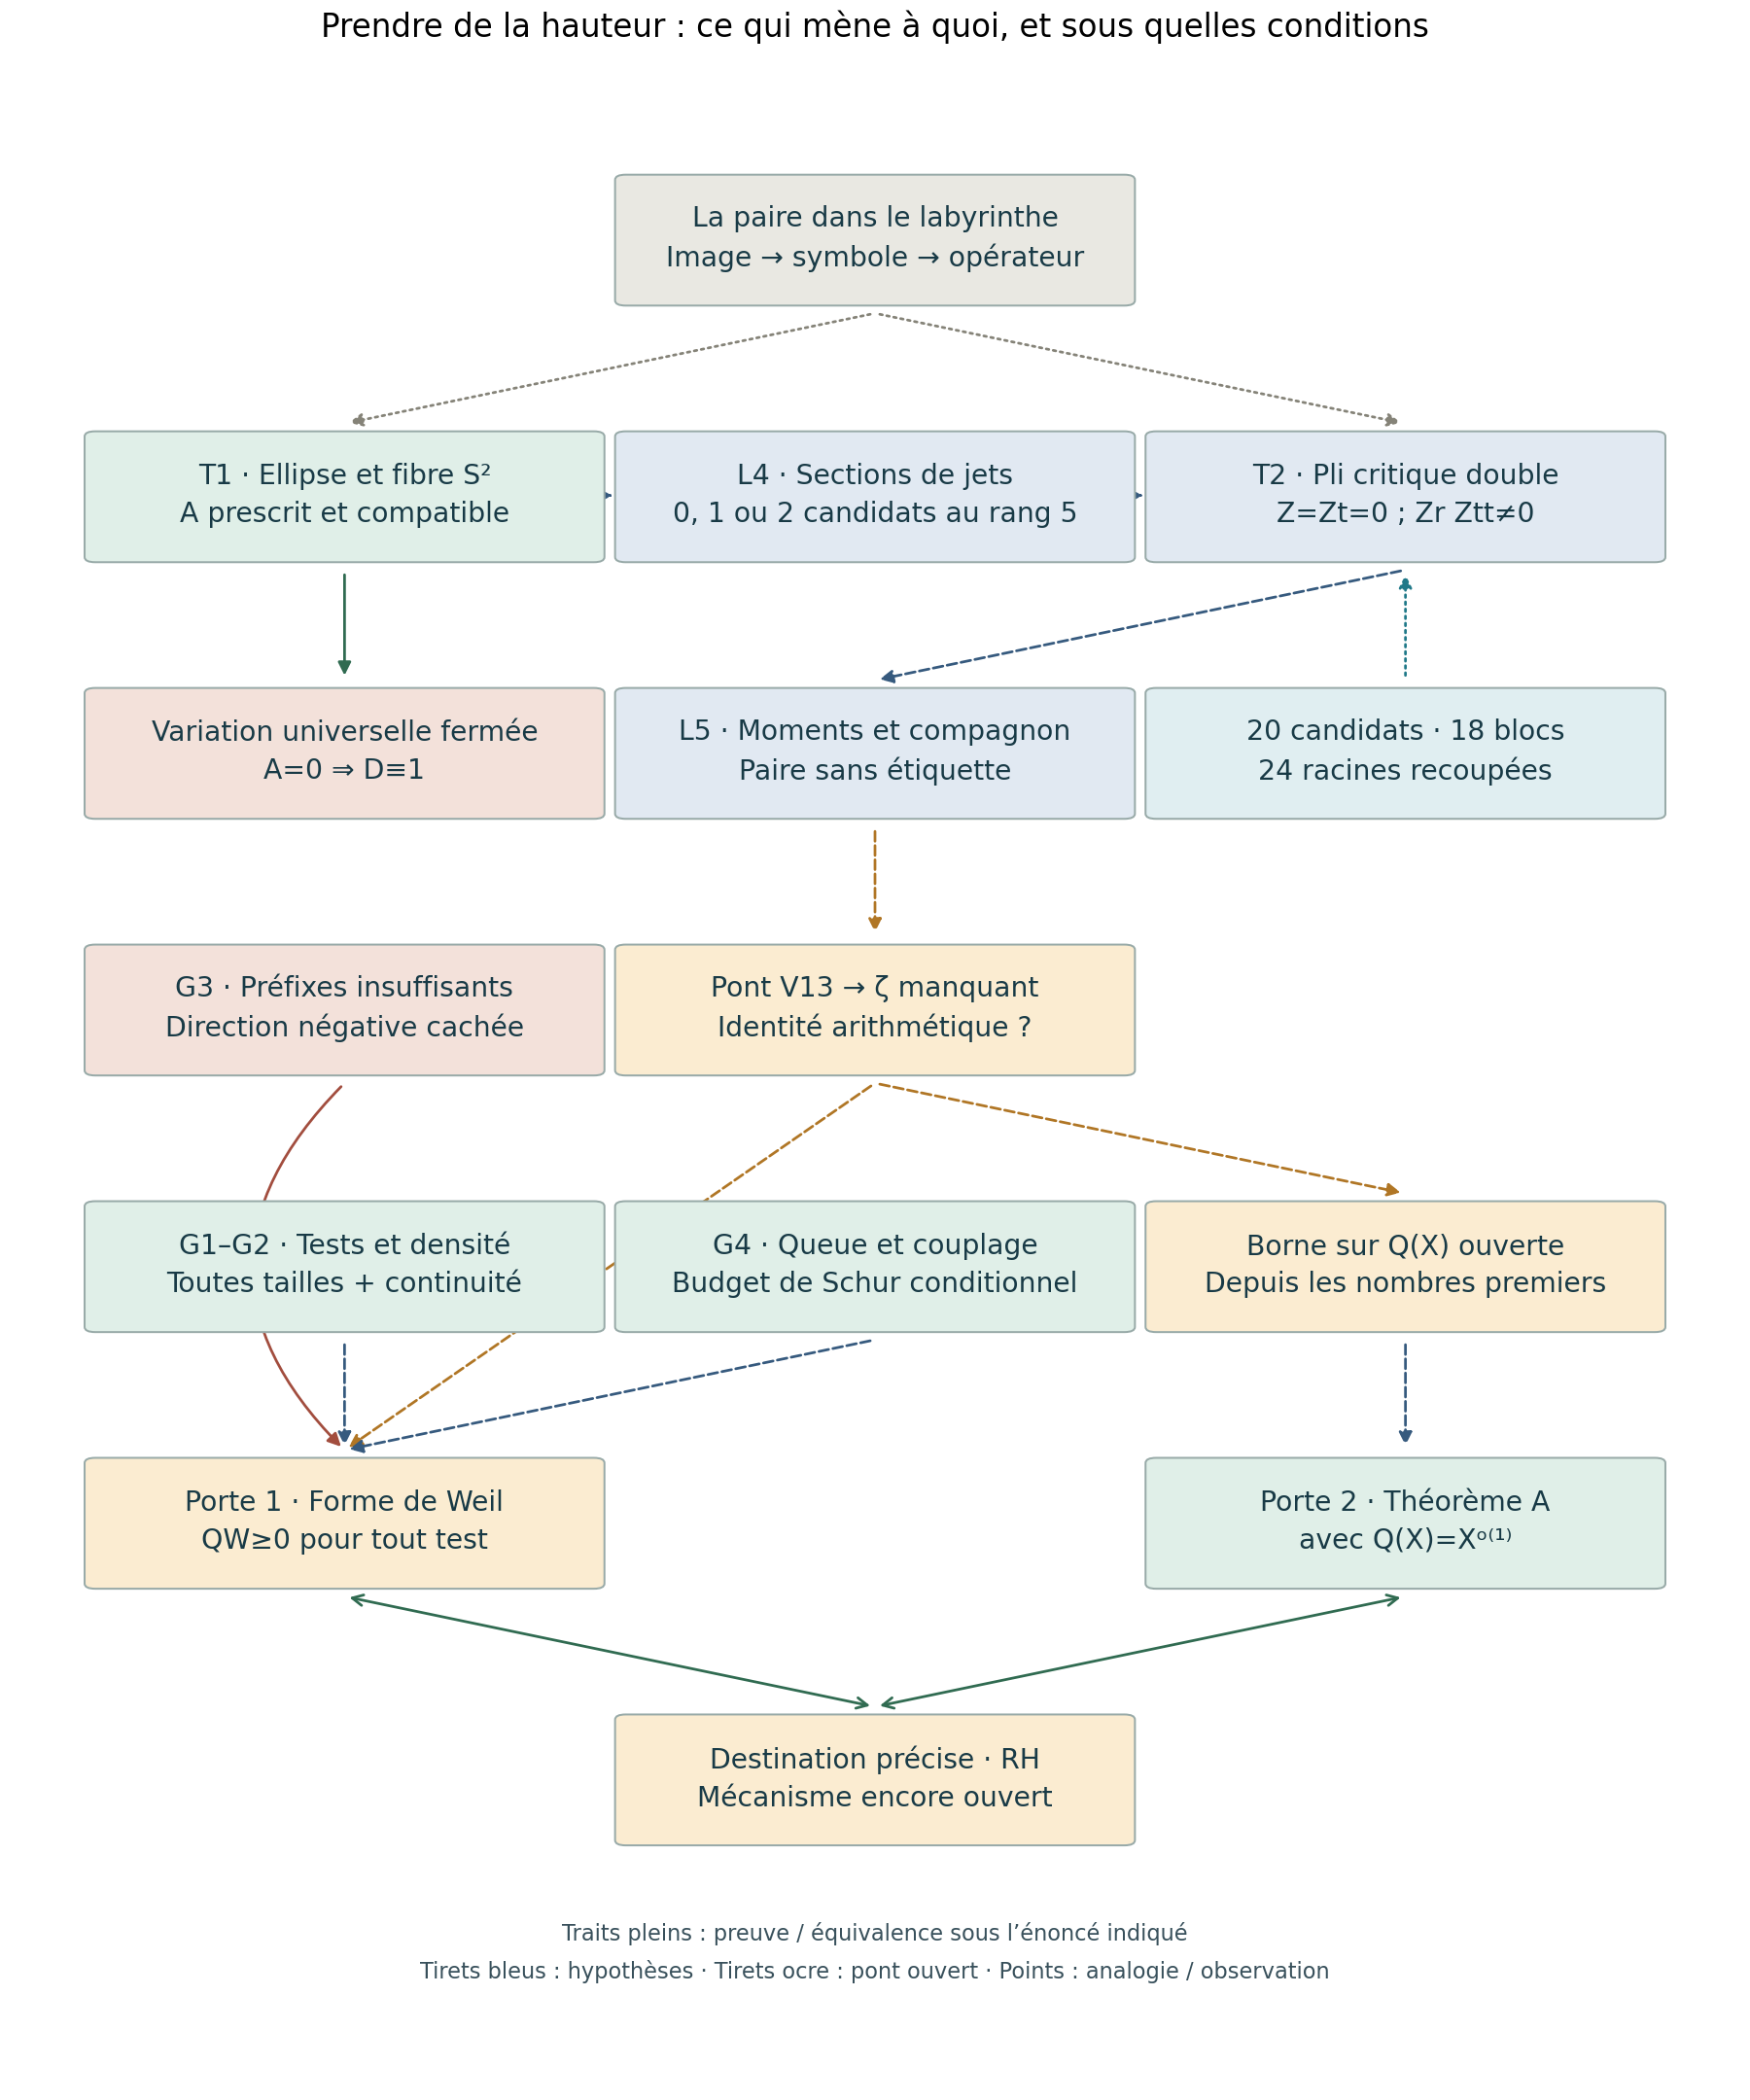
\includegraphics[width=0.85\textwidth,height=\textheight]{65_Graphe_des_passages.png}
\caption{Graphe des idées, énoncés, mesures et obstacles. Les flèches
conditionnelles exigent les hypothèses indiquées ; les ponts ouverts ne
sont pas des implications.}
\end{figure}

Le graphe interactif accompagne ce dossier :
\texttt{65\_GRAPHE\_DES\_PASSAGES.html}. Chaque nœud expose son énoncé,
ses hypothèses, ses relations et sa preuve ou ses données. Le registre
JSON permet de transformer la carte sans confondre une analogie, une
preuve, une observation et une question ouverte.

\newpage

\hypertarget{du-coefficient-complexe-uxe0-une-guxe9omuxe9trie-calculable}{%
\subsection{3. Du coefficient complexe à une géométrie
calculable}\label{du-coefficient-complexe-uxe0-une-guxe9omuxe9trie-calculable}}

La famille V13 emploie les six caractères impairs modulo 13, indexés par
\(k=1,3,5,7,9,11\). Leurs phases exactes \(z_j\), de module 1, viennent
des sommes finies de Gauss et de la normalisation de l'équation
fonctionnelle. Les coefficients réels \(c_j\) vérifient \(\|c\|=1\) et
\(A=\sum_jc_jz_j\). La carte étudiée fixe une ancre positive
\(c_i=\cos r\), avec \(0<r<\pi/4\), donc une ancre unique. Le cas
\(r=0\) et une ancre négative demandent une autre carte.

Écrire \(c=\cos r\,e_i+\sin r\,u\), \(u_i=0\), \(\|u\|=1\). Sur les cinq
coordonnées hors ancre, poser

\[
M_i=\begin{pmatrix}(\Re z_j)_{j\ne i}\\(\Im z_j)_{j\ne i}\end{pmatrix},
\quad G_i=M_iM_i^T,
\quad b={1\over\sin r}\binom{\Re(A-\cos r\,z_i)}{\Im(A-\cos r\,z_i)}.
\]

Le rang de \(M_i\) est deux dans les recettes V13. Pour un \(A\)
prescrit, définir \(u_0=M_i^TG_i^{-1}b\) et \(\eta=b^TG_i^{-1}b\).

\textbf{Théorème T1 --- Faisabilité exacte.} La fibre est vide si
\(\eta>1\), réduite à un point si \(\eta=1\), et une sphère affine
\(S^2\) si \(\eta<1\) :

\[
c=\cos r\,e_i+\sin r\left(u_0+\sqrt{1-\eta}\,Nv\right),
\qquad v\in S^2,
\]

où \(N:\mathbb R^3\to\ker M_i\) est une isométrie, avec réinsertion de
la coordonnée nulle de l'ancre.

\textbf{Preuve.} \(M_iM_i^TG_i^{-1}=I_2\), donc \(M_iu_0=b\). La
solution \(u_0\) appartient à l'image de \(M_i^T\), orthogonale au
noyau. Toute solution est \(u_0+w\), \(w\in\ker M_i\), et
\(\|u_0+w\|^2=\eta+\|w\|^2\). Le noyau a dimension trois : la norme
impose \(\|w\|^2=1-\eta\), d'où les trois cas. □

Les cibles réalisables forment une ellipse pleine centrée en
\(\cos r\,z_i\), de demi-axes \(\sin r\sqrt{\lambda_j(G_i)}\). C'est le
sens exact de « A arbitraire » : toute cible prescrite est examinable,
puis son accessibilité est décidée. Le projecteur du noyau est
\(I-M_i^TG_i^{-1}M_i\) ; le projecteur tangent à une fibre intérieure
est \(N(I-vv^T)N^T\). Ainsi l'image devient un calcul d'opérateurs
explicites.

\begin{figure}
\centering
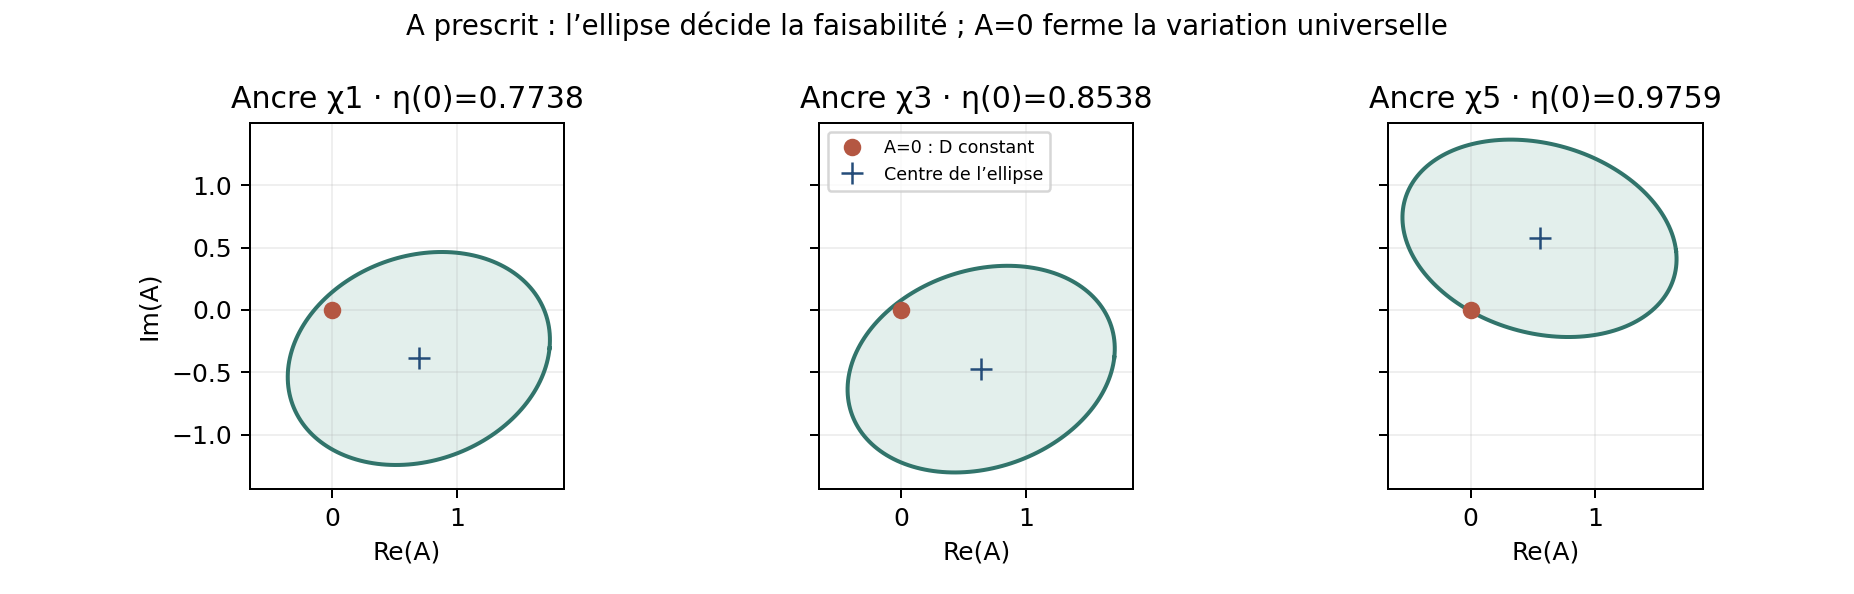
\includegraphics{65_Ellipses_et_fibres.png}
\caption{Ellipses à r=13/20 et A=0 intérieur pour les trois ancres
représentatives. Les phases sont évaluées pour la figure ; les
encadrements de faisabilité sont conservés dans le certificat.}
\end{figure}

\hypertarget{d-devient-une-cubique-une-voie-universelle-est-fermuxe9e}{%
\subsubsection{D devient une cubique ; une voie universelle est
fermée}\label{d-devient-une-cubique-une-voie-universelle-est-fermuxe9e}}

Pour \(\|c\|=1\), le défaut du corpus est

\[
D(c)=1+|A|^2-2\Re\left[A\sum_jc_j^3\overline{z_j}\right].
\]

Sur la fibre, il s'écrit \(D(v)=C+P_1(v)+P_2(v)+P_3(v)\), avec \(P_k\)
homogène de degré \(k\) : une forme linéaire, une matrice symétrique et
un tenseur cubique. Leur formule complète figure dans la note
géométrique.

\textbf{Lemme L2.} D est constant sur la fibre intérieure si et
seulement si \(P_2=q\|v\|^2\) pour un réel q et \(P_3+\|v\|^2P_1=0\)
comme identités polynomiales.

\textbf{Preuve.} Comparer \(v\) et \(-v\) sur la sphère donne
\(P_1+P_3=0\). Par homogénéité, cette égalité équivaut à la seconde
identité pour tout v. La partie paire est constante sur la sphère si et
seulement si la matrice de \(P_2\) est scalaire. La réciproque résulte
des mêmes identités. □

À \(A=0\), \textbf{D≡1 exactement}. À \(r=13/20\), ce cas est intérieur
pour les six ancres ; les représentants ont les encadrements suivants :

\begin{longtable}[]{@{}ll@{}}
\toprule\noalign{}
Ancre & \(\eta(A=0)\), encadrement \\
\midrule\noalign{}
\endhead
\bottomrule\noalign{}
\endlastfoot
χ1 & {[}0,773778141912 ; 0,773778141913{]} \\
χ3 & {[}0,853767785835 ; 0,853767785836{]} \\
χ5 & {[}0,975929422513 ; 0,975929422514{]} \\
\end{longtable}

Les ancres conjuguées donnent les mêmes valeurs. Au bord \(\eta=1\),
aucun couple distinct ne peut être construit. Ces deux contreexemples
réfutent une variation pour toute cible compatible.

\textbf{Variation générique.} Les conditions de constance dépendent
réellement analytiquement de A à l'intérieur. Elles ne sont pas
identiquement satisfaites, puisque V6.39 démontre une variation au
centre pour chaque ancre et rayon. Leur lieu commun d'annulation est
donc fermé sans intérieur ; son complément est ouvert et dense. Cette
conclusion n'est pas une variation universelle.

\textbf{Lemme L3 --- Borne de contraction.}
\(\sup D-\inf D\le12\sin^3 r\,|A|\sqrt{1-\eta}\). En effet, pour
\(h(u)=\sum_{j\ne i}\Re(A\overline z_j)u_j^3\) sur la boule unité,
\(\|\nabla h\|\le3|A|\). D a une constante de Lipschitz \(6\sin^3r|A|\)
; le diamètre de la fibre en u vaut \(2\sqrt{1-\eta}\). Cela prouve la
borne et explique la disparition du contraste près de A=0 ou du bord. □

\newpage

\hypertarget{les-jets-un-filtre-compatible-puis-un-pli-sous-conditions}{%
\subsection{4. Les jets : un filtre compatible, puis un pli sous
conditions}\label{les-jets-un-filtre-compatible-puis-un-pli-sous-conditions}}

Les fonctions de Hardy \(Z_j(t)\) ont une normalisation commune réelle
sur la droite critique. Alors \(Z_c(t)=\sum_jc_jZ_j(t)\). À une hauteur
t fixée, empiler les cinq contraintes :

\[
C_i(t)=\begin{pmatrix}e_i^T\\\Re z^T\\\Im z^T\\Z(t)^T\\Z'(t)^T\end{pmatrix},
\qquad b_i=\begin{pmatrix}\cos r\\\Re A\\\Im A\\0\\0\end{pmatrix}.
\]

\textbf{Lemme L4.} Si \(\operatorname{rang}C_i=5\), poser
\(c_0=C_i^T(C_iC_i^T)^{-1}b_i\), \(\nu=\|c_0\|^2\) et choisir un vecteur
unitaire n du noyau. Les solutions normalisées sont deux points
\(c_0\pm\sqrt{1-\nu}\,n\) si \(\nu<1\), un point si \(\nu=1\), aucune si
\(\nu>1\).

\textbf{Preuve.} \(c_0\) est orthogonal au noyau, qui a dimension un.
Toute solution vaut \(c_0+\alpha n\) et sa norme carrée vaut
\(\nu+\alpha^2\). □

À rang \(q<5\), vérifier d'abord \(b_i\in\operatorname{Im}C_i\) : si
cette compatibilité tient, la même preuve donne une sphère \(S^{5-q}\)
pour \(\nu<1\). Une matrice de Gram singulière ne doit pas être
inversée. Un candidat satisfait une multiplicité au moins deux ; il faut
encore \(Z_c''\ne0\) pour une multiplicité exactement deux et une
transversalité dans le paramètre pour un pli.

\textbf{Bilan du plan fixé.} Les 120 lignes géométriques donnent 72
intérieures, 24 frontières à tolérance et 24 extérieures. Les lignes de
centre sont répétées par les deux axes : ce n'est pas un ensemble de 120
réplications indépendantes. Les 36 sections testent χ1, χ3, χ5 ;
t=5,10,15,20 ; \(\eta=0,1/4,1\) ; \(r=\pi/6\). Deux sections donnent
quatre candidats :

\begin{longtable}[]{@{}
  >{\raggedright\arraybackslash}p{(\columnwidth - 6\tabcolsep) * \real{0.2500}}
  >{\raggedright\arraybackslash}p{(\columnwidth - 6\tabcolsep) * \real{0.2500}}
  >{\raggedleft\arraybackslash}p{(\columnwidth - 6\tabcolsep) * \real{0.2500}}
  >{\raggedright\arraybackslash}p{(\columnwidth - 6\tabcolsep) * \real{0.2500}}@{}}
\toprule\noalign{}
\begin{minipage}[b]{\linewidth}\raggedright
Ancre et hauteur
\end{minipage} & \begin{minipage}[b]{\linewidth}\raggedright
A testé
\end{minipage} & \begin{minipage}[b]{\linewidth}\raggedleft
\(\nu\) numérique
\end{minipage} & \begin{minipage}[b]{\linewidth}\raggedright
\(Z_{tt}\) des deux candidats
\end{minipage} \\
\midrule\noalign{}
\endhead
\bottomrule\noalign{}
\endlastfoot
χ1, t=5 & Centre de l'ellipse & 0,8288412580 & 1,8221119005 ;
1,8594343625 \\
χ3, t=15 & Centre de l'ellipse & 0,9382168857 & −1,8333902743 ;
−2,0420694137 \\
\end{longtable}

Les 34 autres sections sont vides selon le diagnostic numérique ; aucune
absence pour toute hauteur ou toute cible A n'en résulte. Les rangs et
jets de cette étape utilisent Euler--Maclaurin et des différences
centrées sans borne d'erreur : ce sont des candidats, pas des collisions
certifiées.

\hypertarget{thuxe9oruxe8me-t2-le-pli-critique-double}{%
\subsubsection{Théorème T2 --- Le pli critique
double}\label{thuxe9oruxe8me-t2-le-pli-critique-double}}

Soit \(Z(r,t)\) réel analytique, avec prolongement holomorphe local.
Supposer \(Z=Z_t=0\) en \((r_*,t_*)\) et \(Z_rZ_{tt}\ne0\). La
préparation de Weierstrass donne, pour \(h=r-r_*\) et \(x=t-t_*\),

\[
Z=U(h,x)\,[x^2+a_1(h)x+a_0(h)]
 =U(h,x)\,[\xi^2-\mu(h)],\qquad \xi=x+a_1(h)/2,
\]

où \(U(0,0)\ne0\), \(a_j(0)=0\), \(\mu=a_1^2/4-a_0\), et

\[
\mu(0)=0,\qquad \mu'(0)=\kappa=-2Z_r/Z_{tt}\ne0.
\]

\textbf{Preuve.} La multiplicité deux en x autorise la préparation. La
réalité rend les coefficients réels pour h réel. Au point double,
\(U(0,0)=Z_{tt}/2\) et \(a_0'(0)=Z_r/U(0,0)\) ; dériver la définition de
\(\mu\) donne la formule. Ainsi \(\mu>0\) donne deux racines critiques
simples, \(\mu<0\) une paire conjuguée en hauteur complexe, et \(\mu=0\)
un zéro double. Le jacobien du système \((Z,Z_t)\) vaut \(Z_rZ_{tt}\),
donc le point de collision est isolé localement. □

Le jet de Hasse d'ordre deux est ici le jet de Taylor divisé par les
factorielles : \(Z_rh+\tfrac12Z_{tt}x^2+\cdots\). Son modèle
\(x^2\simeq\kappa h\) est une approximation ; \(\kappa h\) n'est pas le
discriminant exact à rayon fini. Aucun de ces énoncés n'est une
assertion sur tous les zéros de la famille.

\newpage

\hypertarget{traverser-la-collision-sans-perdre-la-paire}{%
\subsection{5. Traverser la collision sans perdre la
paire}\label{traverser-la-collision-sans-perdre-la-paire}}

Prendre la coordonnée de hauteur \(w=-i(s-1/2)\). Un zéro critique a w
réel ; le partenaire fonctionnel d'un zéro devient son conjugué en w.
Sur un contour contenant exactement deux zéros et aucun pôle, définir

\[
m_k={1\over2\pi i}\oint w^k{F_w\over F}\,dw.
\]

\textbf{Lemme L5 --- Reconstruction sans étiquette.} Avec les
multiplicités, \(m_0=2\), \(m_1=w_1+w_2\), \(m_2=w_1^2+w_2^2\). Ainsi

\[
a=m_1/2,\quad\Delta_w=2m_2-m_1^2=(w_1-w_2)^2,
\quad\mu=\Delta_w/4,
\quad H=\begin{pmatrix}a&1\\\mu&a\end{pmatrix}.
\]

\textbf{Preuve.} Le théorème des résidus donne les sommes de puissances.
L'identité de Newton fournit \(\Delta_w\), et le polynôme
caractéristique de H est \((\lambda-a)^2-\mu\), de racines \(w_1,w_2\).
□

La matrice a un bloc de Jordan au zéro double. Pour a et μ réels,
\(M=\operatorname{diag}(\mu,1)\) vérifie \(H^TM=MH\). Si \(\mu>0\), M
est définie positive ; si \(\mu<0\), elle est indéfinie ; au double,
elle est singulière. La matrice
\(J=\begin{pmatrix}0&1\\1&0\end{pmatrix}\) donne aussi \(H^TJ=JH\) et,
après retrait du centre, \(J(H-aI)=\operatorname{diag}(\mu,1)\).

Cette métrique est reconstruite après connaissance de la paire : elle ne
force pas son signe. Elle n'est pas la forme de Weil pour ζ. Le
changement de variable est essentiel : \(\Delta_s=-\Delta_w\). La
positivité locale de μ est donc à lire en hauteur w. Une perte
d'isolation du contour ou un compte autre que deux invalide ce bloc.

\hypertarget{ruxe9sultats-prospectifs-complets-20-candidats-de-plis}{%
\subsubsection{Résultats prospectifs complets : 20 candidats de
plis}\label{ruxe9sultats-prospectifs-complets-20-candidats-de-plis}}

Le verrou est daté du 12 octobre 2026 à \textbf{14:04:33 UTC}, avant les
nouveaux calculs de zéros. Les douze couples V6.39 et leurs empreintes
sont conservés. Les deux grilles du Wronskien, t∈{[}−25,25{]}, ont les
pas 0,01 et 0,005. Elles repèrent les mêmes 20 candidats dans
0\textless r≤3/4. Tous sont recoupés à 40 et 70 chiffres de travail par
des jets explicites de Hurwitz.

Pour \(Z=\cos r\,X+\varepsilon\sin r\,Y\), \(\varepsilon=\pm1\), le
Wronskien \(W=XY'-X'Y\) annule les candidats ; la recette \texttt{atan2}
choisit le quadrant du rayon. Les cas hors domaine et les rejets sont
conservés. Une grille de changements de signe n'épuise pas tous les
zéros de W.

\begingroup
\renewcommand{\arraystretch}{0.85}

\begin{longtable}[]{@{}
  >{\raggedright\arraybackslash}p{(\columnwidth - 8\tabcolsep) * \real{0.2000}}
  >{\raggedright\arraybackslash}p{(\columnwidth - 8\tabcolsep) * \real{0.2000}}
  >{\raggedleft\arraybackslash}p{(\columnwidth - 8\tabcolsep) * \real{0.2000}}
  >{\raggedleft\arraybackslash}p{(\columnwidth - 8\tabcolsep) * \real{0.2000}}
  >{\raggedleft\arraybackslash}p{(\columnwidth - 8\tabcolsep) * \real{0.2000}}@{}}
\toprule\noalign{}
\begin{minipage}[b]{\linewidth}\raggedright
Ancre
\end{minipage} & \begin{minipage}[b]{\linewidth}\raggedright
Membre
\end{minipage} & \begin{minipage}[b]{\linewidth}\raggedleft
\(r_*\), arrondi
\end{minipage} & \begin{minipage}[b]{\linewidth}\raggedleft
\(t_*\), signe conservé
\end{minipage} & \begin{minipage}[b]{\linewidth}\raggedleft
\(\kappa\), arrondi
\end{minipage} \\
\midrule\noalign{}
\endhead
\bottomrule\noalign{}
\endlastfoot
χ1 & + & 0,379542 & -23,232362 & -0,868355 \\
χ1 & + & 0,495851 & -18,471606 & -0,724397 \\
χ1 & + & 0,326826 & -12,925459 & -2,096158 \\
χ1 & − & 0,251196 & -11,248150 & -1,418202 \\
χ1 & + & 0,243079 & 4,861023 & -1,807990 \\
χ1 & − & 0,687215 & 7,144416 & -2,942602 \\
χ1 & − & 0,445296 & 16,826334 & -0,621803 \\
χ1 & − & 0,692818 & 20,761042 & -0,109771 \\
χ1 & + & 0,509439 & 22,249146 & -1,928301 \\
χ1 & − & 0,521726 & 24,003322 & -0,439486 \\
χ5 & + & 0,322072 & -22,263442 & -0,635690 \\
χ5 & − & 0,582562 & -20,595550 & -1,679269 \\
χ5 & − & 0,567153 & -17,605551 & -1,085578 \\
χ5 & + & 0,488252 & -15,775936 & -1,358266 \\
χ5 & − & 0,266099 & -9,970874 & -1,546240 \\
χ5 & + & 0,686375 & 16,536483 & -0,223400 \\
χ5 & − & 0,417394 & 17,884820 & -1,826411 \\
χ5 & + & 0,280389 & 19,626457 & -1,245852 \\
χ5 & + & 0,466323 & 23,434100 & -0,909082 \\
χ5 & − & 0,198353 & 24,901146 & -1,243768 \\
\end{longtable}

\endgroup

Les 20 valeurs de κ sont négatives dans ce plan. Ce résultat décrit ces
candidats ; ce n'est pas un signe universel pour V13. Résidus petits et
accord entre précisions ne prouvent ni existence et unicité par
intervalles, ni exhaustivité. Deux jets ont également été repris par
\texttt{mp.diff} à 70 chiffres ; ce contrôle utilise le même backend et
reste un recoupement de formule.

\newpage

\hypertarget{branches-changement-denveloppe-et-blocs-numuxe9riques}{%
\subsection{6. Branches, changement d'enveloppe et blocs
numériques}\label{branches-changement-denveloppe-et-blocs-numuxe9riques}}

Six graines héritées des racines V6.40 sont suivies sur les grilles
\(\Delta r=1/200\) et \(1/400\). Les quatre familles sont χ1 et χ5,
membres plus et moins. Les six branches de la grille fine sont
attribuées à six plis par les critères de proximité gelés. Sur la grille
coarse, χ1 plus est perdue au voisinage du pli : cette perte est
conservée, et ne devient ni une absence de zéro ni une continuation
réussie.

\begin{figure}
\centering
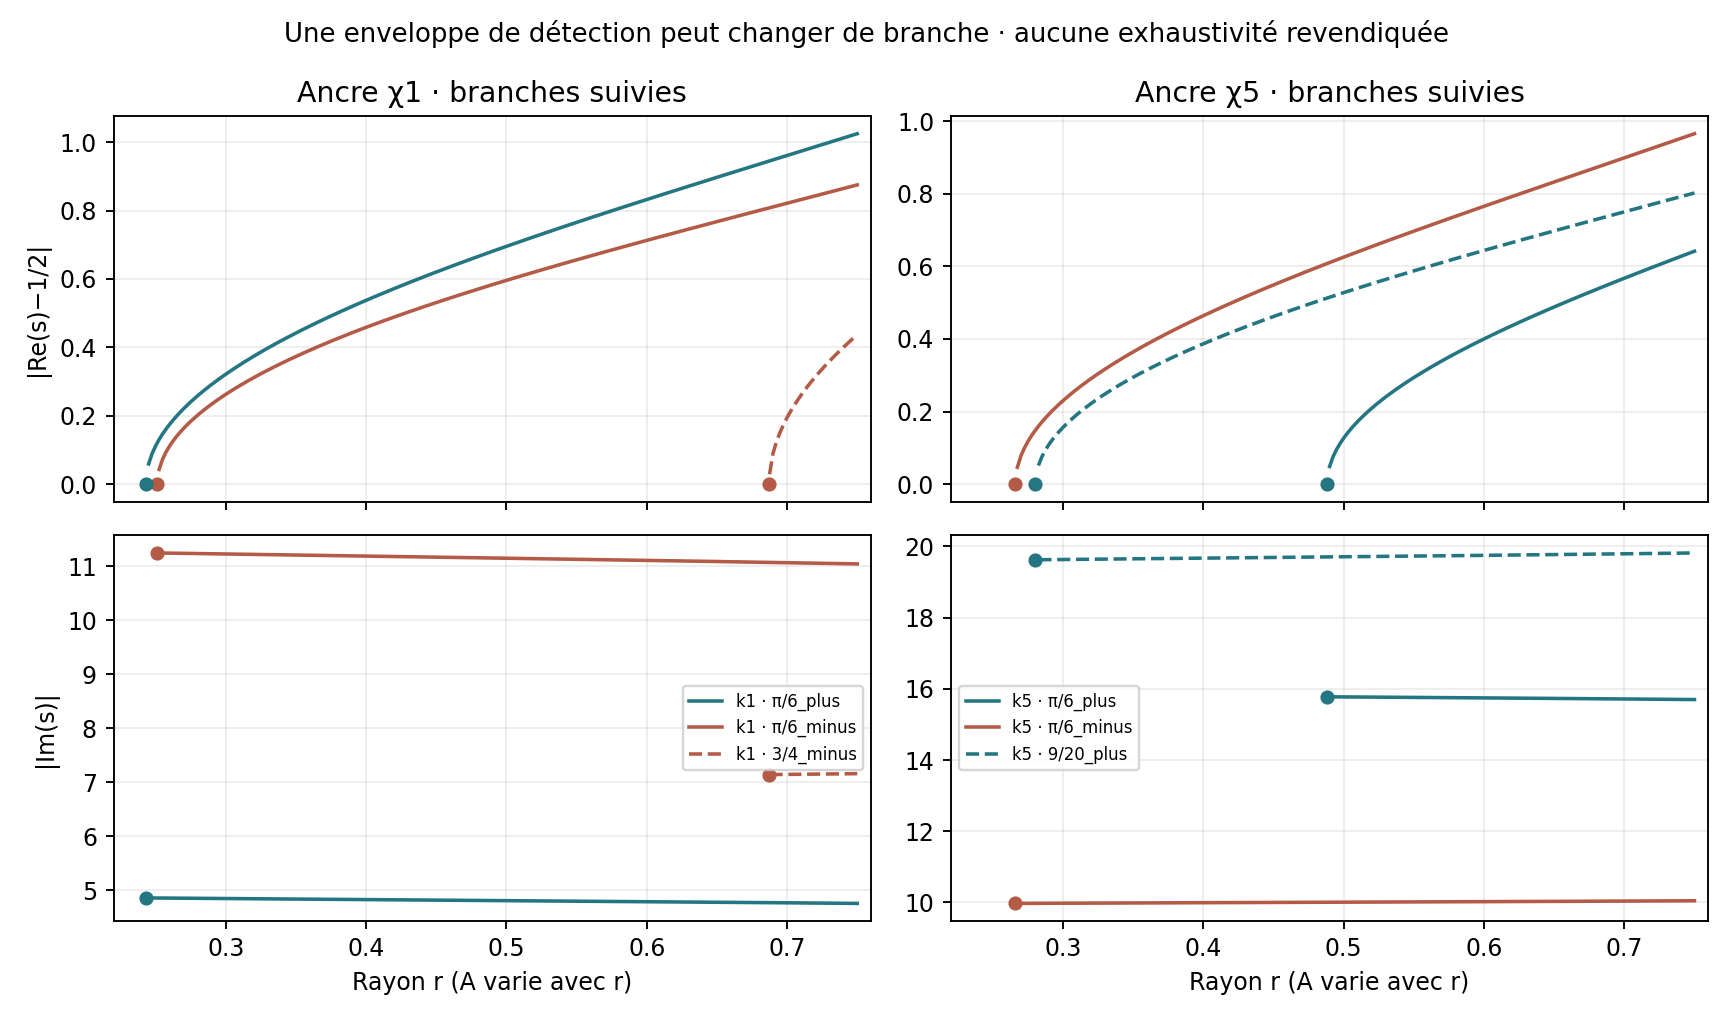
\includegraphics{65_Branches_et_plis.png}
\caption{Les six branches suivies et leurs plis attribués. Les points
sont des localisations numériques ; les lignes relient la continuation
fine. La trajectoire radiale fait varier A.}
\end{figure}

Deux changements de branche éclairent l'enveloppe de détection du
document 64. Pour χ1 moins, la branche de hauteur proche de −11 continue
vers r=3/4, mais une autre branche, née près de r=0,687215 à t=7,144416,
intervient à plus faible \textbar t\textbar. Pour χ5 plus, la branche de
hauteur +19,6 est déjà présente à r=0,45 ; une autre naît près de
r=0,488252 à t=−15,775936 et intervient à plus faible
\textbar t\textbar{} à r=π/6. La première détection peut donc changer de
composante : ce n'est pas le déplacement d'une seule racine étiquetée.

Cette explication porte sur les branches suivies et l'enveloppe
numérique observée. Elle ne certifie pas le vrai premier zéro hors
droite. Les suivis radiaux ne sont pas des déplacements à A constant : A
varie avec r. Les sections de jets de la section 4 répondent séparément
aux contraintes à A fixé.

\hypertarget{blocs-et-24-racines-avec-la-collision-conservuxe9e}{%
\subsubsection{18 blocs et 24 racines, avec la collision
conservée}\label{blocs-et-24-racines-avec-la-collision-conservuxe9e}}

Autour des six plis attribués, les rayons \(r_*−10^{-4}\), \(r_*\),
\(r_*+10^{-4}\) donnent 18 blocs acceptés selon le protocole. Les
cercles en w ont rayon 0,2, avec 128/256 points et deux pas de
différentiation. Les comptes sont proches de deux et les moments
concordent aux seuils gelés. Les 24 racines aux deux rayons latéraux
sont reprises à 40/70 chiffres et distinctes numériquement.

\begin{figure}
\centering
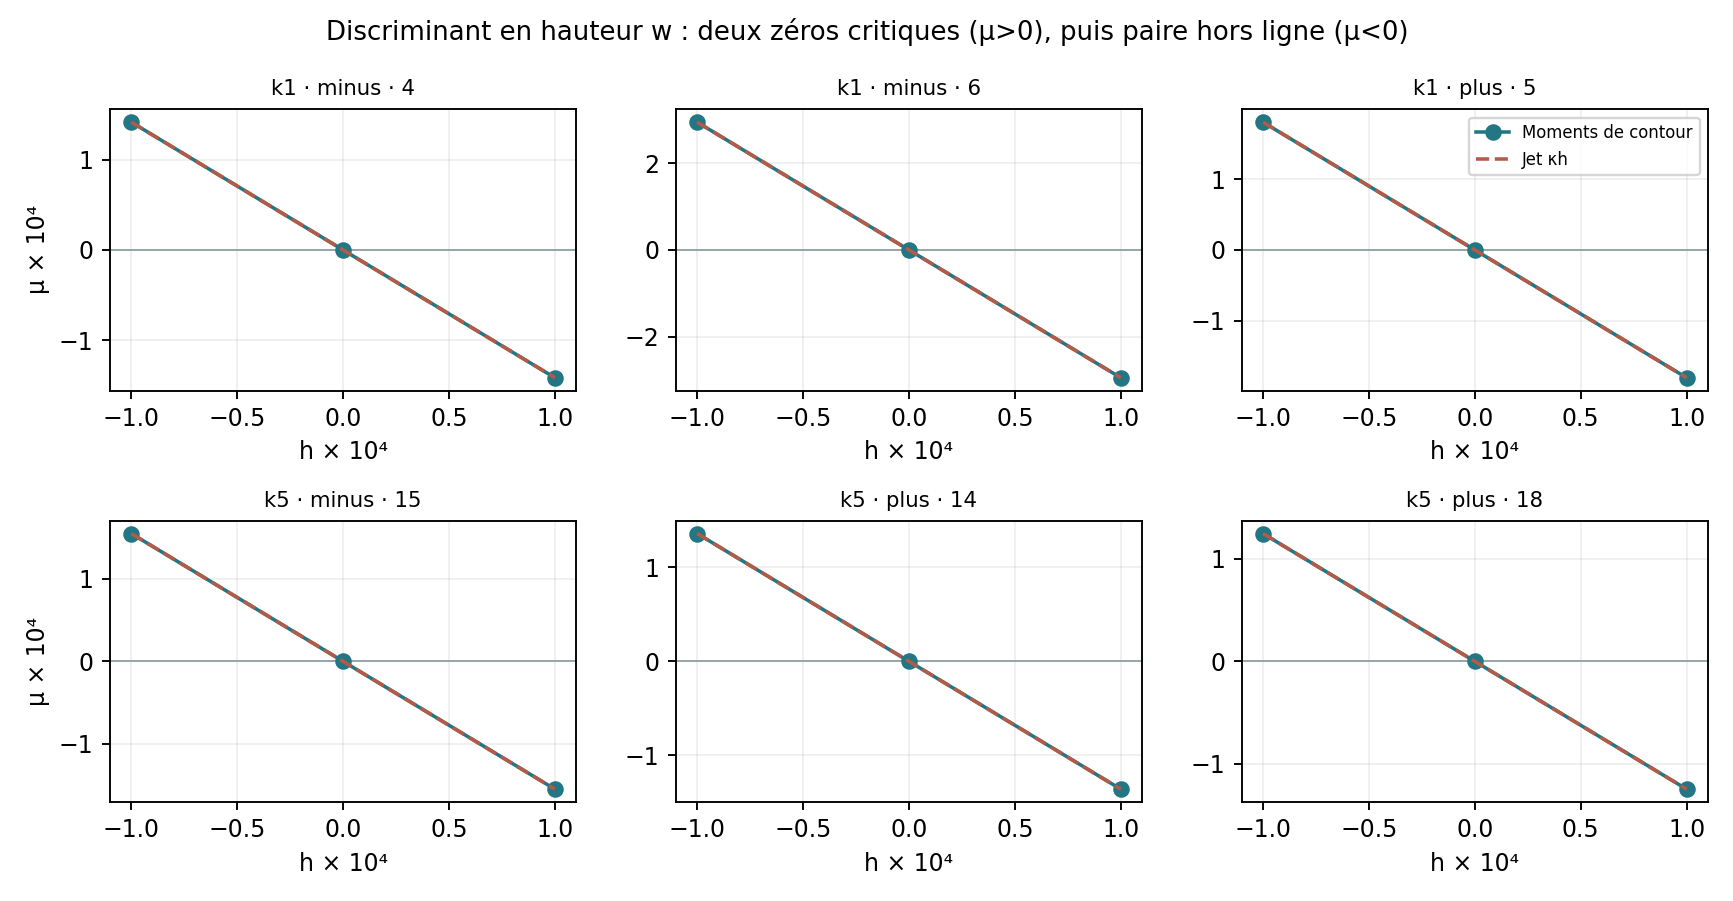
\includegraphics{65_Discriminants_des_paires.png}
\caption{Moments de contour et modèle linéaire du jet autour des six
plis. Au rayon central, un petit discriminant numérique n'est pas
présenté comme une annulation exacte.}
\end{figure}

Avant le pli (\(h<0\)), les six blocs ont \(\Delta_w>0\) et deux racines
critiques ; après (\(h>0\)), \(\Delta_w<0\) et une paire hors ligne. Le
rayon central porte le statut \texttt{near\_collision}, sans imposer μ=0
aux résultats flottants. Les résidus imaginaires des invariants sont
conservés et contrôlés. Les métriques réelles affichées utilisent ces
invariants réels dans le modèle conditionnel ; elles ne certifient pas
leur réalité exacte.

Les minima du bord sont \textbf{échantillonnés}. Sans borne sur tout le
contour, ces données ne démontrent pas qu'il isole exactement deux
zéros. Le bloc de la section 5 est exact sous cette hypothèse ; son
instance numérique reste à certifier.

\hypertarget{unituxe9s-fictives-cohuxe9rentes}{%
\subsubsection{Unités fictives
cohérentes}\label{unituxe9s-fictives-cohuxe9rentes}}

Les coefficients normalisés c, les phases z et D sont sans dimension.
Introduire une unité fictive \(\mathsf C\) pour les coefficients
effectifs \(\mathsf Cc\) : A et F portent alors \(\mathsf C\), et les
dérivées spectrales portent \(\mathsf C/\mathsf T^k\) si w porte une
unité \(\mathsf T\). Les moments \(m_k\) ont l'unité \(\mathsf T^k\) ;
\(\Delta_w\) et μ portent \(\mathsf T^2\). Le rapport \(F_w/F\) élimine
l'unité \(\mathsf C\).

La matrice dimensionnellement homogène est
\(\widetilde H=\begin{pmatrix}a/\mathsf T&1\\\mu/\mathsf T^2&a/\mathsf T\end{pmatrix}\),
avec spectre \(w_j/\mathsf T\) ; l'opérateur \(\mathsf T\widetilde H\)
porte \(\mathsf T\). Une énergie fictive \(\mathsf E D\) porte
\(\mathsf E\) ; sa dérivée par rapport à un temps porte
\(\mathsf E/\mathsf T\). Une énergie positive n'impose pas une dérivée
positive. Ces unités accompagnent les calculs sans identifier un
Hamiltonien physique.

\newpage

\hypertarget{la-porte-globale-tests-limite-queue-et-couplage}{%
\subsection{7. La porte globale : tests, limite, queue et
couplage}\label{la-porte-globale-tests-limite-queue-et-couplage}}

Le critère de Weil publié {[}CC21{]} est indépendant des expériences
V13. Dans la convention Fourier de son introduction, les distributions
locales satisfont RH si et seulement si leur somme est non positive sur
les autocorrélations admissibles. Nous prenons son opposée :

\[
E=\left\{f\in C_c^\infty(\mathbb R):\int f(x)e^{\pm x/2}\,dx=0\right\},
\quad Q_W(f)=-\sum_vW_v(g*g^*),\quad g(u)=f(\log u).
\]

Ici \(g^*(u)=\overline{g(u^{-1})}\), la convolution multiplicative
utilise \(du/u\), et l'involution additive est
\(f^*(x)=\overline{f(-x)}\). Dans cette convention : \(Q_W(f)\ge0\) pour
chaque \(f\in E\) équivaut à RH. Les annulations correspondent aux deux
points polaires. La convention Mellin de l'appendice C emploie un
changement de normalisation ; elle ne se substitue pas terme à terme à
la convention Fourier.

La source fournit le critère global et un résultat archimédien à support
restreint ; ce dernier n'est pas une positivité globale de toute la
forme arithmétique. Notre vérification primaire porte sur le critère et
ses conditions, pas sur une validation de l'article entier.

\hypertarget{lemme-g1-construire-tous-les-tests-admissibles}{%
\subsubsection{Lemme G1 --- Construire tous les tests
admissibles}\label{lemme-g1-construire-tous-les-tests-admissibles}}

Avec \(P=\partial_x^2-1/4\), on a \(E=P C_c^\infty(\mathbb R)\).

\textbf{Preuve.} Deux intégrations par parties donnent
\(\int e^{\pm x/2}P\psi=\int P(e^{\pm x/2})\psi=0\). Réciproquement,
pour \(f\in E\), poser
\(\psi(x)=\int_{-\infty}^x2\sinh((x-y)/2)f(y)\,dy\). La différentiation
donne \(P\psi=f\). À gauche du support, ψ est nulle ; à droite elle vaut
\(e^{x/2}\int e^{-y/2}f(y)dy-e^{-x/2}\int e^{y/2}f(y)dy=0\). Elle est
lisse et compacte. Le noyau de P sur les fonctions compactes est nul,
car une combinaison des deux exponentielles ne peut être compacte. □

L'opérateur élimine les contraintes d'admissibilité. Il n'impose pas le
signe de \(Q_W(P\psi)\).

\hypertarget{lemme-g2-une-hiuxe9rarchie-dense-avec-un-contrat-de-limite}{%
\subsubsection{Lemme G2 --- Une hiérarchie dense, avec un contrat de
limite}\label{lemme-g2-une-hiuxe9rarchie-dense-avec-un-contrat-de-limite}}

Choisir \(\chi_L\in C_c^\infty((-L-1,L+1))\) égale à 1 sur {[}−L,L{]},
et poser

\[
E_{L,N}=\operatorname{span}_{|n|\le N}
P\left(\chi_L(x)e^{in\pi x/(L+1)}\right).
\]

Ces espaces sont inclus dans E et emboîtés en N pour L fixé. Leur
réunion sur L,N est dense dans la topologie des tests.

\textbf{Preuve.} Écrire \(f=P\psi\) par G1 ; choisir L tel que le
support de ψ soit contenu dans (−L,L). Son prolongement périodique de
période 2(L+1) est lisse. Ses sommes de Fourier convergent avec toutes
les dérivées. Multiplier par \(\chi_L\) puis appliquer P donne une
approximation de f, avec support compact commun et convergence de toutes
les dérivées. □

Si une forme hermitienne est continue dans cette topologie et positive
sur \textbf{tous} les \(E_{L,N}\), elle est positive sur E, en passant à
la limite. Pour des compressions approchées, il faut notamment

\[
|Q_W(f_N)-\widetilde Q_{L,N}(f_N)|
\le\varepsilon_{L,N}\|f_N\|_*^2\longrightarrow0,
\]

avec une minoration compatible tendant vers zéro et une norme justifiée.
Cette erreur et cette minoration ne sont pas établies pour ζ dans le
corpus. La densité rend le but précis ; elle ne fournit pas le signe
manquant.

\newpage

\hypertarget{thuxe9oruxe8me-g3-les-seuls-pruxe9fixes-finis-ne-suffisent-pas}{%
\subsubsection{Théorème G3 --- Les seuls préfixes finis ne suffisent
pas}\label{thuxe9oruxe8me-g3-les-seuls-pruxe9fixes-finis-ne-suffisent-pas}}

Pour chaque M, sur \(\ell^2(\mathbb N)\),
\(K_M=I-2|e_{M+1}\rangle\langle e_{M+1}|\) est borné autoadjoint de
norme 1. Ses compressions aux n premières coordonnées sont \(I_n\) pour
\(n\le M\), mais \(\langle e_{M+1},K_Me_{M+1}\rangle=-1\).

\textbf{Preuve.} Le rang un est orthogonal aux M premières coordonnées
et vaut 1 sur \(e_{M+1}\). □

Un procédé ne disposant que de ces préfixes ne distingue donc pas I de
\(K_M\). C'est une impossibilité sur les opérateurs arbitraires avec ces
seules données. Une identité arithmétique ou une borne uniforme peut
changer les hypothèses. \textbf{Ce n'est pas une impossibilité de
prouver RH.}

\hypertarget{lemme-g4-contruxf4ler-la-queue-et-le-couplage}{%
\subsubsection{Lemme G4 --- Contrôler la queue et le
couplage}\label{lemme-g4-contruxf4ler-la-queue-et-le-couplage}}

Pour un opérateur borné autoadjoint
\(K=\begin{pmatrix}\mathcal A&B\\B^*&C\end{pmatrix}\),
\(\mathcal A\ge aI\) avec \(a>0\),

\[
K\ge0\iff C-B^*\mathcal A^{-1}B\ge0.
\]

\textbf{Preuve.} Compléter le carré donne

\[
\langle(x,y),K(x,y)\rangle
=\|\mathcal A^{1/2}(x+\mathcal A^{-1}By)\|^2
+\langle y,(C-B^*\mathcal A^{-1}B)y\rangle.
\]

Choisir \(x=-\mathcal A^{-1}By\) démontre la nécessité ; la même
identité prouve la suffisance. En particulier, \(C\ge cI\), \(c\ge0\) et
\(\|B\|^2\le ac\) suffisent, car \(\mathcal A^{-1}\le a^{-1}I\). □

Il faut les trois estimations : marge du bloc, minoration de la queue,
norme du couplage. Une marge a qui tend vers zéro peut rendre ce budget
insuffisant. Pour une forme non bornée, domaines et fermeture demandent
un autre travail. Nous n'avons pas construit un opérateur K pour ζ
satisfaisant déjà ces hypothèses.

\hypertarget{la-deuxiuxe8me-porte-la-croissance-de-luxe9nergie-arithmuxe9tique}{%
\subsubsection{La deuxième porte : la croissance de l'énergie
arithmétique}\label{la-deuxiuxe8me-porte-la-croissance-de-luxe9nergie-arithmuxe9tique}}

Le théorème A du corpus établit

\[
{1\over2}\limsup_{X\to\infty}{\log(1+Q(X))\over\log X}
=\Theta-{1\over2},\qquad
\mathrm{RH}\iff Q(X)=X^{o(1)}.
\]

Il donne une implication exploitable dès qu'une borne suffisante est
obtenue indépendamment de RH depuis les premiers. La positivité
\(Q(X)\ge0\) ne contrôle pas cette croissance. Le théorème B suppose RH
; l'utiliser pour prouver RH sans lever cette hypothèse serait
circulaire. Ces deux théorèmes gardent leur portée antérieure. La note
65 ajoute des outils et des contre-épreuves, sans ajouter la borne
globale manquante.

\newpage

\hypertarget{les-uxe9tapes-ultuxe9rieures-avec-crituxe8res-darruxeat}{%
\subsection{8. Les étapes ultérieures, avec critères
d'arrêt}\label{les-uxe9tapes-ultuxe9rieures-avec-crituxe8res-darruxeat}}

\begin{longtable}[]{@{}
  >{\raggedright\arraybackslash}p{(\columnwidth - 4\tabcolsep) * \real{0.3333}}
  >{\raggedright\arraybackslash}p{(\columnwidth - 4\tabcolsep) * \real{0.3333}}
  >{\raggedright\arraybackslash}p{(\columnwidth - 4\tabcolsep) * \real{0.3333}}@{}}
\toprule\noalign{}
\begin{minipage}[b]{\linewidth}\raggedright
Étape
\end{minipage} & \begin{minipage}[b]{\linewidth}\raggedright
Travail à réaliser
\end{minipage} & \begin{minipage}[b]{\linewidth}\raggedright
Condition de réussite ou conclusion utile
\end{minipage} \\
\midrule\noalign{}
\endhead
\bottomrule\noalign{}
\endlastfoot
1. Certifier un pli local & Choisir avant calcul un des six plis
attribués ; jet analytique, boîte rationnelle, Newton/Krawczyk par
intervalles ; contour continu & Existence et unicité dans la boîte,
\(Z_rZ_{tt}\ne0\), deux zéros isolés ; sinon obstacle chiffré
conservé \\
2. Déployer à A fixé & Choisir une des deux sections de jets faisables ;
paramétrer une géodésique de la fibre exacte ; tester la transversalité
& Collision et paramètre compatibles avec A, ancre et rayon constants ;
sinon rang, dégénérescence ou incompatibilité identifiés \\
3. Fixer la porte globale & Spécifier la forme arithmétique, le domaine
et la topologie ; construire la hiérarchie G1--G2 et l'expression depuis
les premiers & Un contrat de signe ou de croissance écrit sans supposer
RH ; absence du pont explicitement démontrée si les objets diffèrent \\
4. Chercher l'inégalité manquante & Minorer la queue et borner le
couplage, ou majorer Q(X) de façon uniforme & Hypothèses et
quantificateurs établis ; sinon témoin négatif ou limite de méthode \\
\end{longtable}

Ces étapes sont des programmes de recherche, pas des résultats déjà
obtenus. Les nouveaux calculs devront être précédés d'un nouveau verrou
: aucune sélection postérieure parmi les quatre candidats de jets n'est
présentée comme une prévision réalisée. L'extension du seul plafond ne
répond à aucun des contrats globaux.

Le modèle Bellman courant ajoute aux neuf actions historiques : le
dossier de passages V13, achevé ; la certification d'un bloc local ;
l'audit du contrat global. Coûts H et utilités U sont conventionnels. Un
rapport concluant à un obstacle compte comme livrable, sans recevoir le
statut de preuve de RH. Les ex aequo sont conservés. Le calcul optimise
le modèle documentaire déclaré, pas les chances de résoudre un problème
ouvert.

\begin{figure}
\centering
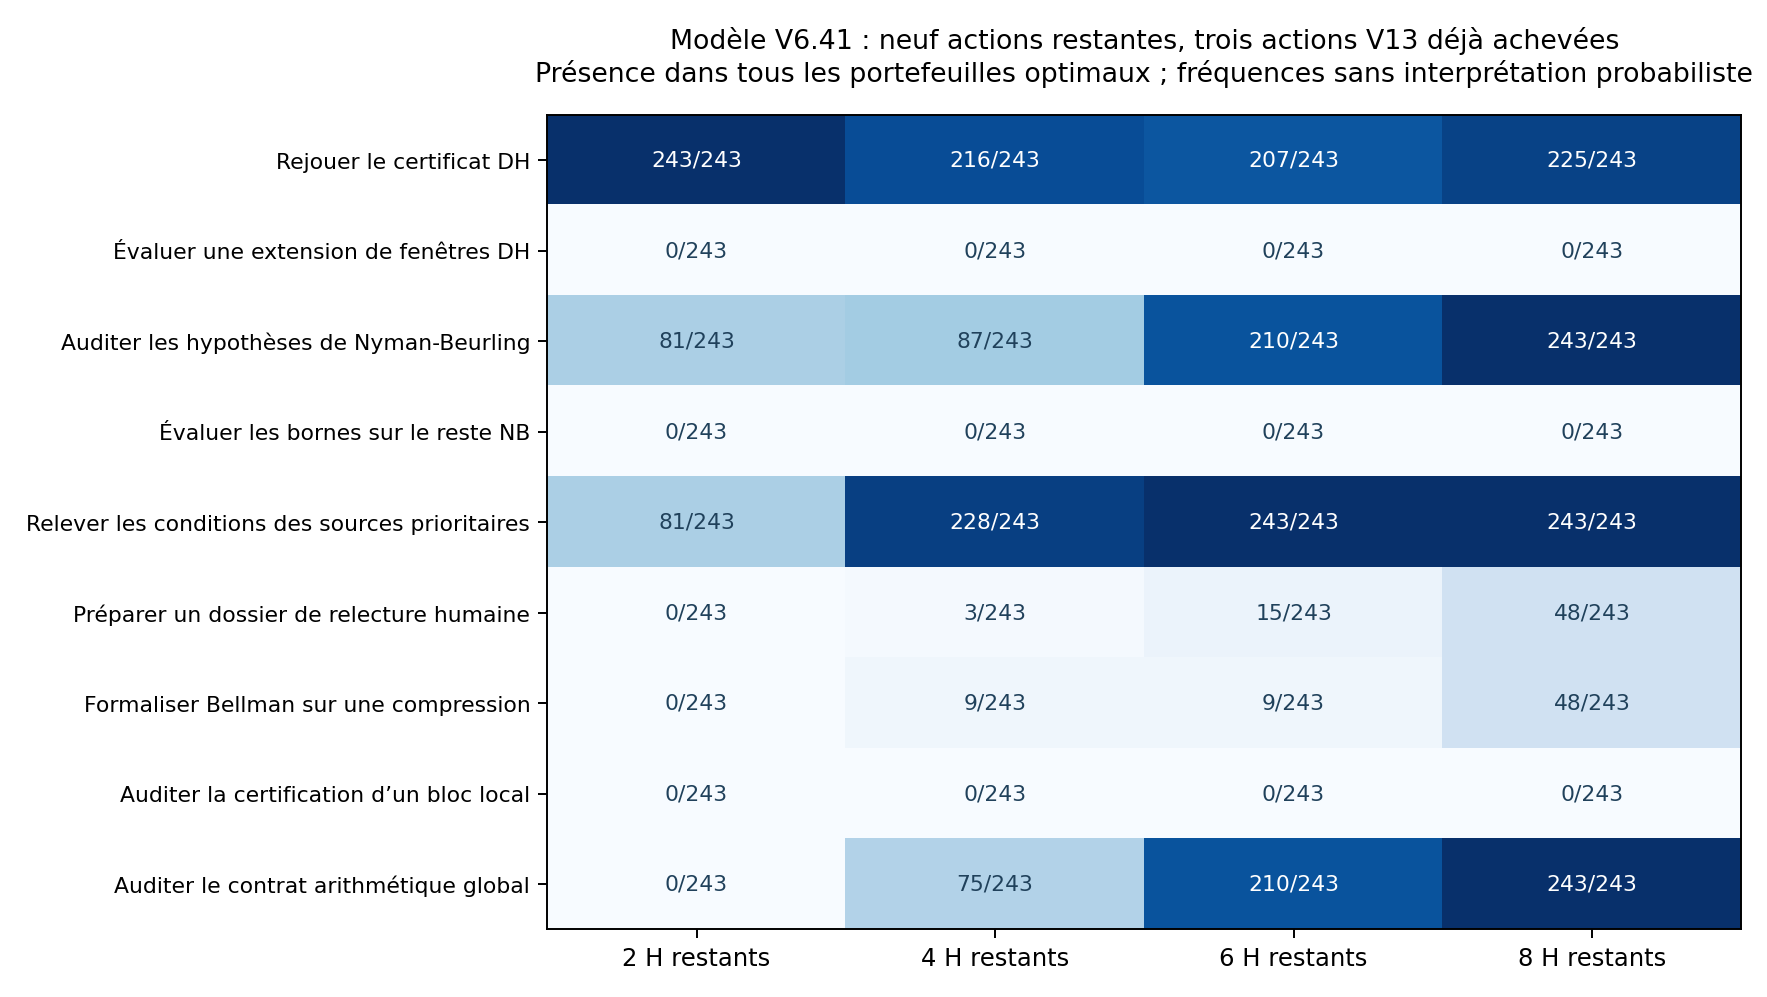
\includegraphics{65_Bellman_sensibilite.png}
\caption{Modèle courant : neuf actions restantes après les trois actions
V13 achevées. La fréquence sur 243 profils est une sensibilité aux poids
conventionnels, pas une probabilité de succès.}
\end{figure}

\hypertarget{sources-preuves-et-reproduction}{%
\subsection{9. Sources, preuves et
reproduction}\label{sources-preuves-et-reproduction}}

\textbf{{[}CC21{]}} A. Connes et C. Consani, \emph{Weil positivity and
Trace formula, the archimedean place} (2021), introduction (4),
appendices A--C et proposition C.1.
\href{https://alainconnes.org/wp-content/uploads/Selecta.pdf}{PDF
auteur} ; \href{https://arxiv.org/abs/2006.13771}{prépublication}.
Vérification primaire du critère, de l'involution et du changement de
normalisation ; validation de l'ensemble de l'article non revendiquée.

Les résultats de fibres, jets et plis sont démontrés dans les trois
notes ci-dessous. Les préparations de Weierstrass, résidus,
pseudo-inverses et compléments de Schur sont des outils classiques ;
aucune nouveauté générale de ces outils n'est revendiquée. Le résultat
de recherche ici est leur assemblage explicite, ses restrictions, ses
contreexemples et le protocole appliqué aux familles exactes du corpus.

\begin{longtable}[]{@{}
  >{\raggedright\arraybackslash}p{(\columnwidth - 2\tabcolsep) * \real{0.5000}}
  >{\raggedright\arraybackslash}p{(\columnwidth - 2\tabcolsep) * \real{0.5000}}@{}}
\toprule\noalign{}
\begin{minipage}[b]{\linewidth}\raggedright
Chemin relatif à \texttt{3\_Preuves\_et\_calculs}
\end{minipage} & \begin{minipage}[b]{\linewidth}\raggedright
Contenu
\end{minipage} \\
\midrule\noalign{}
\endhead
\bottomrule\noalign{}
\endlastfoot
\texttt{preuves/V641\_GEOMETRIE\_ET\_OPERATEURS.md} & Fibres, cubique,
constance, contractions, sections de jets et audit constructif \\
\texttt{preuves/V641\_COLLISIONS\_ET\_LIMITES.md} & Wronskien, pli,
moments, opérateurs, audit critique \\
\texttt{preuves/V641\_PASSAGE\_AU\_GLOBAL.md} & G1--G4, signe Weil et
deux portes globales \\
\texttt{data/v641\_protocole\_verrouille.json} & Empreintes, graines et
seuils antérieurs aux calculs \\
\texttt{data/v641\_branches.json} & Deux grilles, six graines et perte
conservée \\
\texttt{data/v641\_wronskiens.json} & Toutes les détections et tous les
rejets \\
\texttt{data/v641\_collisions.json} & Les 20 recoupements et 11
attributions de grille à six plis \\
\texttt{data/v641\_blocs\_paires.json} & 18 blocs, moments, marges
échantillonnées, 24 racines \\
\texttt{data/v641\_geometrie.json} & 120 lignes géométriques et 36
sections de jets \\
\texttt{data/v641\_certificat\_fibres.json} & Intervalles des phases et
faisabilité de A=0 \\
\texttt{data/v641\_graphe\_recherche.json} & Nœuds, statuts, preuves et
types de flèches \\
\end{longtable}

Pour rejouer, travailler sur une copie et déplacer les sorties de la
phase concernée : le lanceur refuse de les écraser. Le manifeste V6.39,
les données V6.40 et les prévisions originales sont conservés. Les
nouvelles notes de lecture suivent l'encodage Markdown du corpus ; les
reçus originaux restent inchangés dans \texttt{4\_Archives/recus/V641}.

\begin{Shaded}
\begin{Highlighting}[]
\BuiltInTok{cd}\NormalTok{ 3\_Preuves\_et\_calculs}
\ExtensionTok{python}\NormalTok{ scripts/run\_v641\_passages.py }\AttributeTok{{-}{-}phase}\NormalTok{ branches}
\ExtensionTok{python}\NormalTok{ scripts/run\_v641\_passages.py }\AttributeTok{{-}{-}phase}\NormalTok{ scan}
\ExtensionTok{python}\NormalTok{ scripts/run\_v641\_passages.py }\AttributeTok{{-}{-}phase}\NormalTok{ collisions}
\ExtensionTok{python}\NormalTok{ scripts/run\_v641\_passages.py }\AttributeTok{{-}{-}phase}\NormalTok{ blocks}
\ExtensionTok{python}\NormalTok{ scripts/run\_v641\_passages.py }\AttributeTok{{-}{-}phase}\NormalTok{ geometry}
\ExtensionTok{python}\NormalTok{ tests/run\_all\_tests.py}
\BuiltInTok{cd}\NormalTok{ ..}
\ExtensionTok{python}\NormalTok{ 2\_Methode/Outils/build\_v641\_graph.py}
\ExtensionTok{python}\NormalTok{ 2\_Methode/Outils/build\_v641\_document.py}
\end{Highlighting}
\end{Shaded}

Dépendances : NumPy, SciPy, pandas, mpmath 1.3.0 ; figures Matplotlib ;
PDF Pandoc et XeLaTeX. Les jets d'ordre deux utilisent les dérivées de
Hurwitz explicites. Le raccourci
\texttt{mpmath.dirichlet(...,\ derivative=2)} n'est pas employé : cette
version ne fournit pas ce contrat, même si elle accepte l'argument. Les
tests comparent les jets à des différentiations numériques.

Le portail, les sources, la carte, la matrice, l'indicateur, le
navigateur, l'atlas et la liste des figures donnent le bilan V6.41. Les
états et PDF historiques restent identifiés comme tels. Les niveaux de
maturité RH ne montent pas du fait d'un nouveau graphe ou d'un nouveau
recoupement local.

\hypertarget{ruxe9fuxe9rences}{%
\subsection{Références}\label{ruxe9fuxe9rences}}

Format : {[}clé{]} auteurs, \emph{titre}, publication, lien. Fiches
complètes et état de vérification : document 42 (registre des sources).

\begin{itemize}
\tightlist
\item
  {[}CC21{]} A. Connes, C. Consani. \emph{Weil positivity and Trace
  formula, the archimedean place}. PDF auteur daté du 4 juillet 2021 ;
  arXiv:2006.13771.
  \url{https://alainconnes.org/wp-content/uploads/Selecta.pdf} ---
  partiellement vérifié
\end{itemize}

\end{document}
